\section{Resultados con materiales reales: Au y Ag}
\label{section:AuAg}

Con la finalidad de presentar la respuesta óptica de una monocapa de NPs conformadas por materiales realista, se emplea en esta sección la función dieléctrica con corrección por tamaño para NPs esféricas de oro [Fig. \ref{sfig:sizeAu}] y de plata [Fig. \ref{sfig:sizeAg}]. La elección de NPs de oro y plata surge a partir de su uso en el biosensado \cite{jain2008noble}, así como por su biocompatibilidad \cite{fan2009bio,bosetti2002silver}. Los cálculos realizados corresponden a la reflectancia y transmitancia en configuración ATR, puesto que en el análisis con las funciones dieléctrica tipo Drude fue en donde se observó la presencia de un modo distinto a las excitaciones de partículas individuales. Asimismo, se realizó el análisis de la transmitancia para corroborar que las excitaciones presentes para materiales realistas presentan un comportamiento semejante al modo guiado reportado en \cite{kabashin2009plasmonic} y \cite{danilov2018ultra}, también observado en sistemas de NPs desordenadas con una función dieléctrica tipo Drude.

En la Fig.  \ref{fig:Au-R-Theta} se muestran los cálculos de la reflectancia $R$, empleando el CSM, de una monocapa de NPs esféricas idénticas de oro con un radio de $a = 25$ nm, inmersa en una matriz de agua ($n_m = 1.5$) y soportada por un sustrato con un índice de refracción $n_s = 1.5$, que es iluminada por una onda plana en una configuración ATR. La reflectancia se grafica como función del ángulo de incidencia $\theta_i$ y tanto de la longitud de onda $\lambda$ (escala inferior), como de la energía en unidades de $\hbar\omega$ (escala superior). Se consideraron las fracciones de cubierta $\Theta = 0.1,\,0.125,\,0.15$ y $0.2$  (garantizando la condición de una muestra diluida para el CSM), así como la polarización de la onda plana incidente: las gráficas \textbf{i)}--\textbf{iv)} corresponden a la polarización \emph{p} y \textbf{v)}--\textbf{viii)} a \emph{s}. Las líneas punteadas verticales verdes y rosas corresponden a las SP-SPRs dipolares y cuadrupolares, respectivamente: para el una NP de oro de $a= 25$ nm inmersa en agua, la SP-SPR dipolar se localiza en $\lambda = 531$ nm y la cuadrupolar en $513$ nm, como se observa en la Fig. \ref{fig:Au-R-Theta}. Los puntos amarillos corresponden al modo colectivo.

	\begin{figure}[h!]\centering
\begin{tikzpicture}
\node[inner sep=0pt] (graf) at (-.1,0){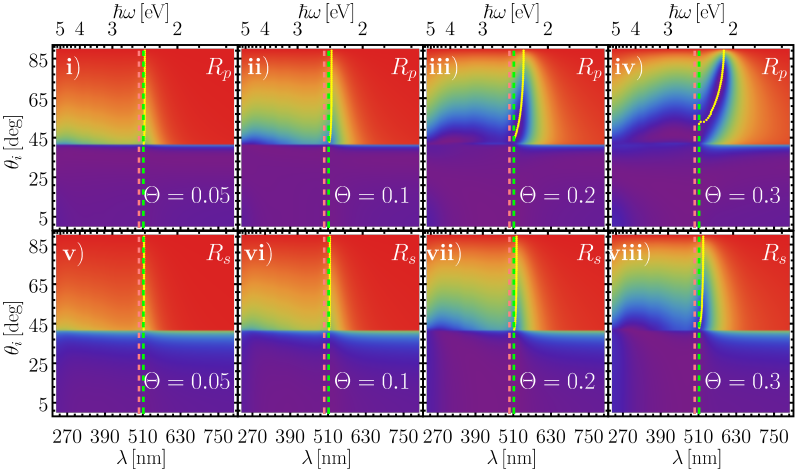
\includegraphics[width = .9\linewidth]{2-Resultados/figs/6-AuThetaVar/0-2D_Grid}};
\node[right, inner sep=0pt] (legend) at (7,.05) {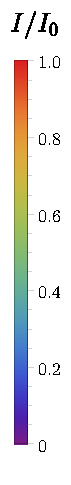
\includegraphics[scale=.77, trim={00 00 00 00}, clip]{2-Resultados/figs/0-IBar_v}};
\node[above, inner sep=0pt] (r) at (7.15,3.2) {$R$};
\end{tikzpicture}\vspace*{-.5em}
	\caption{Gráficas de reflectancia de una monocapa de NPs esféricas de oro de radio $a=25$ nm en configuración ATR como función del ángulo de incidencia $\theta_i$ y de la longitud de onda $\lambda$ (escala inferior), así como de la energía del haz incidente en unidades de $\hbar\omega$ (escala superior).  Las gráficas   en el renglón superior [$\mathbf{i)-v)}$] muestran los resultados para  polarización \emph{p} y las del renglón inferior  [$\mathbf{vi)-x)}$]  para polarización  \emph{s}, donde se consideraron los valores de fracción de cubierta $\Theta =  0.1,\,0.125,\,0.15$ y $0.2$.  Las líneas verticales punteadas verdes y rosas corresponden a las SP-SPRs dipolar en $\lambda=531$ nm y  cuadrupolar en $\lambda=513$, respectivamente.  Los puntos amarillos corresponden a los mínimos en $R$ para ángulos mayores a $\theta_c\approx 62.5^\circ$ y longitudes de onda mayores a la SP-SPRs dipolar.
}	\label{fig:Au-R-Theta}	
	\end{figure}	

A diferencia de los cálculos de la reflectacia de una monocapa de NPs  con una función dieléctrica tipo Drude analizada en la sección \ref{ssection:DrudeATR}, en donde sólo se presentaron excitaciones al rededor de las SP-SPRs y el modo colectivo a longitudes de onda mayores a las de las SP-SPRs, los cálculos de la monocapa de NPs de de oro muestran excitaciones a valores de $\lambda$ menores a las de las SP-SPRs (líneas verticales punteadas), las cuales corresponden a excitaciones no plasmónicas, es decir, a contribuciones de transiciones de electrones ligados. Sin embargo, dado que el modo colectivo se excita a energías menores a las de las transiciones interbanda, su contribución no afecta a la excitación colectiva y ésta aún es apreciable. Para ambas polarizaciones, en las gráficas \textbf{i)}, \textbf{ii)}, \textbf{vi)} y \textbf{vii)}, correspondientes a $\Theta=0.1$ y $0.15$, el modo colectivo tiende a la SP-SPR dipolar para ángulos de incidencia cercanos al ángulo crítico $\theta_c$, sin embargo para valores de $\Theta$ mayores, no es apreciable ningún mínimo cerca $\theta_c$; por ejemplo para $\Theta=0.2$ para polarización \emph{p} a $\lambda = 531$ nm (línea punteada vertical verde) hay un mínimo en la reflectancia a $\theta\approx 75^\circ$, mientras que para \emph{s} lo hay en $65^\circ$. La excitación colectiva para el oro para polarización \emph{p} no tiende a la longitud de onda del SP-SPR dipolar para $\theta_i\approx\theta_c$ debido al ensanchamiento de otras resonancias al crecer la cantidad de material que conforma la monocapa, es decir aumentar la fracción de cubierta, razón por la que se traslapan las resonancias.  Que la polarización \emph{s} el modo colectivo tenga un comportamiento más semejante al de las SP-SPR dipolares, comparado a \emph{p}, concuerda con el comportamiento observado para el análisis de NPs con una función dieléctrica tipo Drude.

La reflectancia de una monocapa de NPs con las mismas características que las de la Fig. \ref{fig:Au-R-Theta} pero con NP esféricas de plata de radio $a=35$ nm (para poder sintonizar las resonancias más cerca del espectro visible), se grafica en la Fig. \ref{fig:Ag-R-Theta}, en donde la SP-SPR dipolar corresponde a la línea vertical verde en $\lambda=430$ nm y la cuadrupolar, a la líneas vertical rosa en $\lambda=375$ nm. Al igual que para la monocapa de NPs de oro, se aprecian excitaciones no plasmónicas en valores de $\lambda$ menores a la de las SP-SPRs sin embargo, para la plata estas excitaciones están separadas de las plasmónicas, como se observa por la presencia de la región roja, al rededor de los $350$ nm,  en donde $R\approx 1$. 

\begin{figure}[h!]\centering
\begin{tikzpicture}
\node[inner sep=0pt] (graf) at (-.1,0){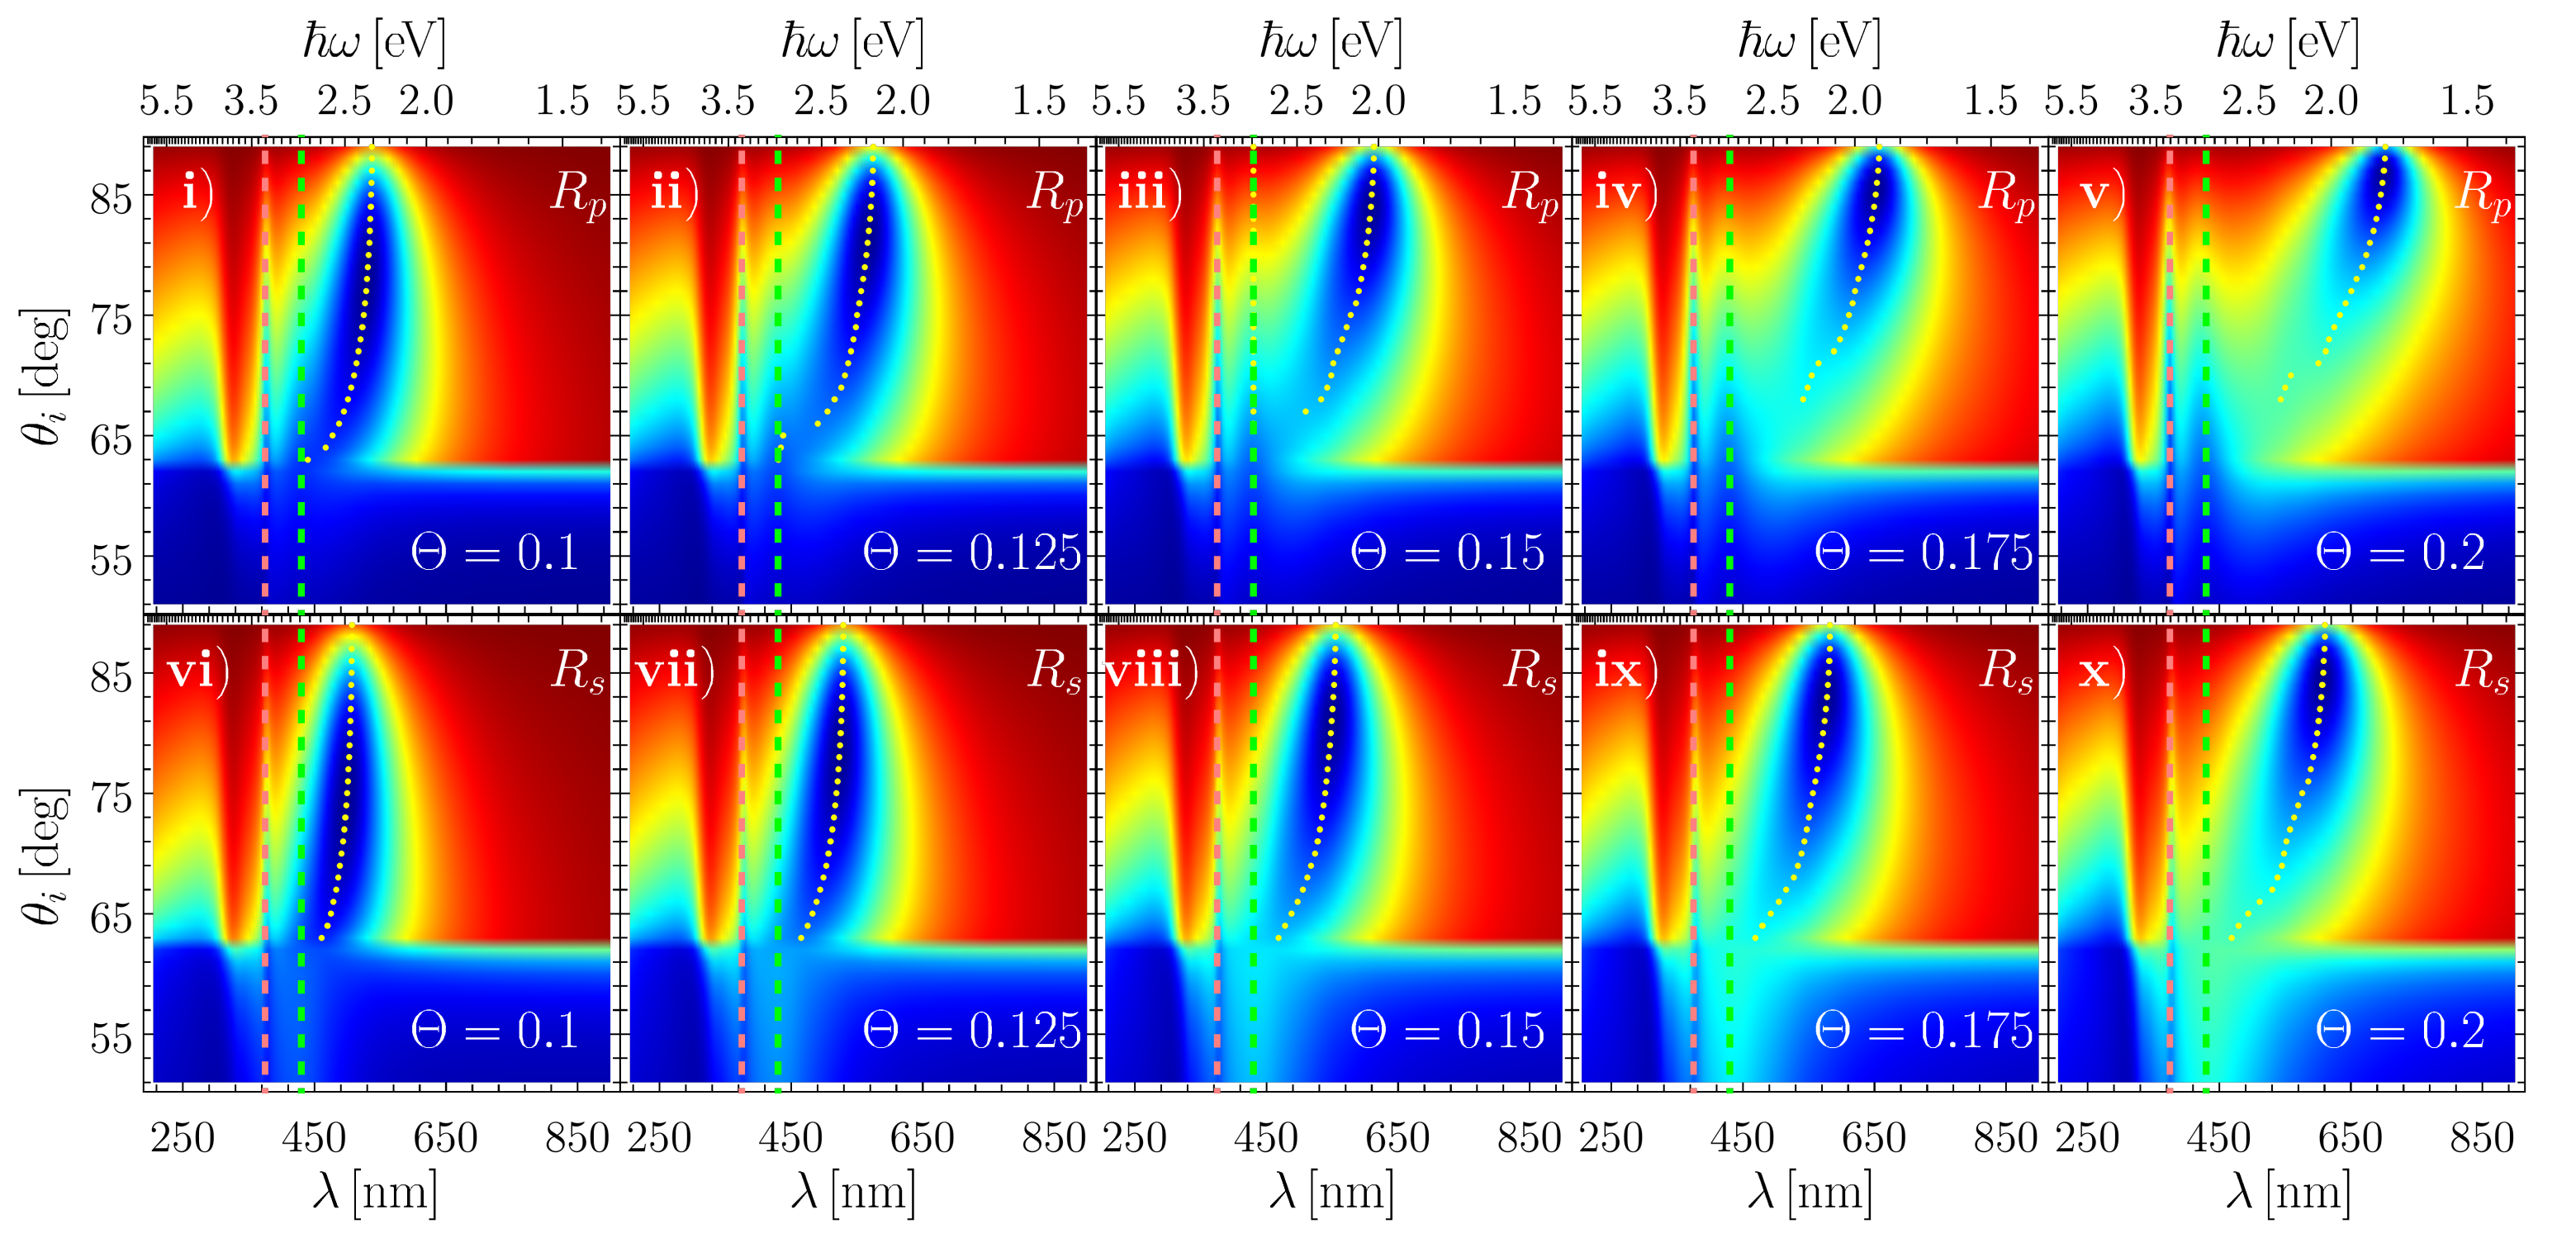
\includegraphics[width = .9\linewidth]{2-Resultados/figs/7-AgThetaVar/0-2D_Grid}};
\node[right, inner sep=0pt] (legend) at (7,.05) {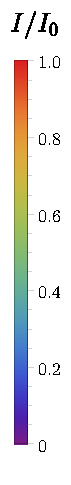
\includegraphics[scale=.78, trim={00 00 00 00}, clip]{2-Resultados/figs/0-IBar_v}};
\node[above, inner sep=0pt] (r) at (7.15,3.2) {$R$};
\end{tikzpicture}\vspace*{-.5em}
	\caption{Gráficas de reflectancia de una monocapa de NPs esféricas de plata de radio $a=35$ nm en configuración ATR como función del ángulo de incidencia $\theta_i$ y de la longitud de onda $\lambda$ (escala inferior), así como de la energía del haz incidente en unidades de $\hbar\omega$ (escala superior).  Las gráficas   en el renglón superior [$\mathbf{i)-v)}$] muestran los resultados para  polarización \emph{p} y las del renglón inferior  [$\mathbf{vi)-x)}$]  para polarización  \emph{s}, donde se consideraron los valores de fracción de cubierta $\Theta = 0.1,\,0.125,\,0.15$ y $0.2$.  Las líneas verticales punteadas verdes y rosas corresponden a las SP-SPRs dipolar en $\lambda=430$ nm y  cuadrupolar en $\lambda=375$, respectivamente.  Los puntos amarillos corresponden a los mínimos en $R$ para ángulos mayores a $\theta_c\approx 62.5^\circ$ y longitudes de onda mayores a la SP-SPRs dipolar.
}	\label{fig:Ag-R-Theta}	
	\end{figure}	

Para una monocapa de NPs de plata, el modo colectivo también es apreciable, al igual que con el oro o con NPs con una función dieléctrico tipo Drude, siendo más parecida su respuesta al de las últimas. Como para la plata las excitaciones no plasmónicas están más alejadas de las SP-SPRs, en comparación con el oro, la resonancia dipolar de partícula individual (línea punteada vertical verde) se aprecia para polarización \emph{p} para fracciones de cubierta mayores a $0.125$ [gráficas \textbf{ii)--\textbf{v)}}], mientras que para polarización \emph{s}, la SP-SPR dipolar no es apreciable para ningún valor de $\Theta$; la SP-SPR cuadrupolar (línea punteada vertical rosa) es apreciable para todos los valores de $\Theta$ a ambas polarizaciones. Otra semejanza entre la monocapa de NPs de plata y la de NPs cuya función dieléctrica está dada por el modelo de Drude, es el límite del modo colectivo cuando $\theta_i$ tiende a $\theta_c$, en donde la longitud de onda de excitación corresponde del modo colectivo corresponde a la de la SP-SPR dipolar.

Tanto para la monocapa de NPs de oro, como de plata, la reflectancia a las longitudes de onda del modo colectivo (puntos amarillos en las Figs. \ref{fig:Au-R-Theta} y \ref{fig:Au-R-Theta}) para un valor de $\Theta$ y $a$ fijos, es menor para ángulos de incidencia rasantes ($\theta_i\lessapprox 90^\circ$).  Adicionalemnte, el ancho de la resonancia a ángulos rasantes es menor en comparación a ángulos menores a $80^\circ$ por lo que localizar al modo colectivo, y emplearlos en el biosensado, sería más en sencillo. Sin embargo, en la medición experimental de la reflectancia, el área del haz empleado se deforma al incidir a la interfaz entre sustrato y la matriz/monocapa de NPs como $A=A'/\cos\theta_i$, en donde $A$ es el área del haz al incidir en la interfaz entre el sustrato y la matriz/monocapa de NPs, y $A'$ es la sección transversal del haz antes de incidir en la interfaz  (ver Fig. \ref{fig:hazcircular}), por lo que el área de sensado se extiende. Para emplear al modo colectivo en el sensado, se restringe el valor de $\theta_i\leq 80^\circ$, en donde el área aumenta en un factor de $5.7$.

Dentro de los cálculos de la reflectancia de las monocapas de NPs de oro y de plata, una diferencia es el valor de $\theta_i$ al cual se comienza a excitar el modo colectivo, una vez escogido $\Theta$, que en el caso del oro para $\Theta=0.15$ es a $\theta_i\approx 65^\circ$. Para analizar este comportamiento, se grafican en la Fig. \ref{fig:AuAg-Cuts-65} cortes de la reflectancia graficada en las Figs. \ref{fig:Au-R-Theta} (para las NPs de oro) y \ref{fig:Ag-R-Theta} (para las de plata) a $\theta_i=65^\circ$. Asimismo, se grafican en la Fig. \ref{fig:AuAg-Cuts-75} cortes de la reflectancia para ambas monocapas a $\theta_i=75^\circ$, ángulo que deforma el área del haz en un factor de $3.8$ y en donde  la reflectancia, evaluada a las longitudes de onda del modo colectivo para todos los casos de $\Theta$ estudiados en las Figs.  \ref{fig:Au-R-Theta} y  \ref{fig:Ag-R-Theta}, es menor a $0.4$, permitiendo que el modo colectivo sea empleado en biosensores. En ambas figuras, los paneles izquierdos corresponden a los cálculos para la monocapa de NPs de oro y los derechos a los de NPs de plata, mientras que los paneles superiores corresponden a la reflectancia en polarización \emph{p} y los inferiores a polarización \emph{s}. Las líneas punteadas verticales verdes corresponden a la SP-SPR dipolar que para las NP de oro se localiza a $531$ nm y para las de plata a $430$ nm; la SP-SPR cuadrupolar (líneas punteadas verticales rosas) se localizan a $513$ nm y a $370$ nm para las NPs de oro y plata, respectivamente.

\begin{figure}[h!]\centering
	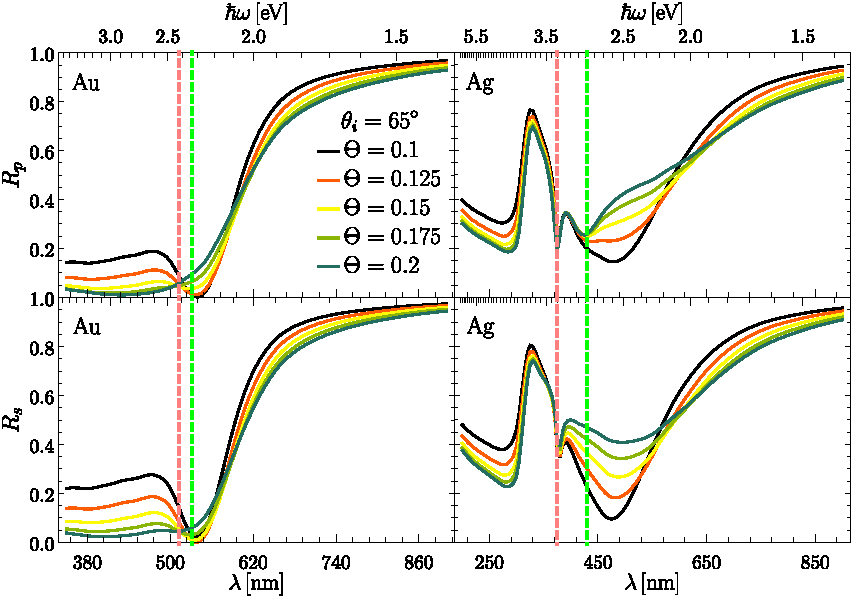
\includegraphics[scale=1]{2-Resultados/figs/6-AuThetaVar/0-cut65_Au_Aug.pdf}\vspace*{-.5em}
	\caption{Cortes a $\theta_i = 65^\circ$ de las gráficas de reflectancia  en configuración ATR  de una monocapa de NPs esféricas de oro de radio $a=25$ nm (Fig. \ref{fig:Au-R-Theta}) y de plta de $a=35$ nm (Fig. \ref{fig:Au-R-Theta}) como función de la longitud de onda $\lambda$ (escalainferior) y de la energía $\hbar\omega$ (escala superior). Los paneles izquierdos corresponden a los cálculos para la monocapa de NPs de oro y los derechos a los de NPs de plata; los panles superiores corresponden a la reflectancia en polarización \emph{p} y los inferiores a polarización \emph{s}. La SP-SPR dipolar (líneas punteadas verticales verdes) para la NP de oro se localiza a $531$ nm y la de la NP de plata a $430$ nm, mientras la SP-SPR cuadrupolar (líneas punteadas verticales rosas) se localizan a $513$ nm y a $370$ nm para las NPs de oro y plara, respectivamente. }\label{fig:AuAg-Cuts-65}
	\end{figure}	
	
%Tanto para la monocapa de NPs de oro como de plata, la reflectancia a valores de $\lambda$ menores a los de la SP-SPR cuadrupolar es menor conforme la fracción de cubierta crece y este comportamiento se invierte para $\lambda$ mayores a la SP-SPR cuadrupolar.
En la Fig. \ref{fig:AuAg-Cuts-65} la reflectancia  para el oro a $\Theta=0.2$  (línea  sólida turquesa) a ambas polarizaciones no presenta la excitación del modo plasmónico a $\lambda>531$ nm y tampoco lo hace a $\Theta=0.175$ para polarización \emph{p} pero sí para polarización \emph{s}, en donde la longitud de onda de excitación del modo colectivo corresponde con la de la SP-SPR dipolar. Al considerar $\Theta= 0.1$ (línea negra)  y $0.125$ (línea naranja)  se cumple que la longitud de onda de excitación del modo colectivo es $\lambda^{exc} = 540\text {nm}$ y que la reflectancia a evaluada en $\lambda^{exc}$ es $R_p\approx0$, mientras que  para polarización \emph{s} con $\Theta=0.1$ se cumple que $R_s(\lambda^{exc}) \approx0.02$ y, para $\Theta=0.125$, $R_s(\lambda^{exc})\approx 0$; para los valores intermedios de $\Theta$ la reflectancia a las longitudes de onda del modo colectivo comienza a aumentar.

Para la monocapa de NPs de plata, la reflectancia a $\theta_i=65^\circ$, a todos los valroes de $\Theta$, presenta un mínimo a $370$ nm (línea punteada vertical rosa) que corresponde a la SP-SPR cuadrupolar para las NPs de plata empleadas. La excitación dipolar de partícula individual a $430$ nm sólo es apreciable como mínimos en la reflectancia a polarización \emph{p} con $\Theta \geq 0.15$, para valores de fracción de cubierta menores, y para polarización \emph{s}, esta excitación puede observarse, no como un mínimo en $R$, sino como un punto estacionario, es decir, el modo colectivo y la SP-SPR dipolar se empalman, cambiando la forma del pico de ambas resonancias. Los valores de reflectancia para la monocapa de NPs de plata considerando $\theta_i=65^\circ$ son mayores al aumentar $\Theta$, y siempre mayores a $0.2$ a diferencia de los resultados con NPs de oro en donde se obtuvieron valores cercanos a cero. Adicionalmente el modo colectivo se corre al rojo al crecer $\Theta$, comportamiento observado en los resultados con NPs con una función dieléctrica tipo Drude pero que no es apreciable para la reflectancia  a  $65^\circ$ de una monocapa de NPs de oro.	
	
	\begin{figure}[h!]\centering
	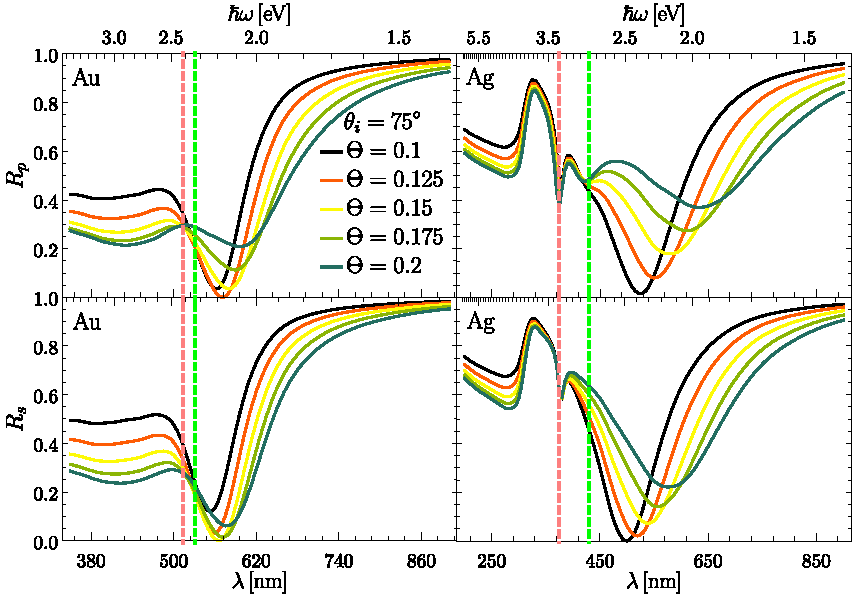
\includegraphics[scale=1]{2-Resultados/figs/6-AuThetaVar/0-cut75_Au_Aug.pdf}\vspace*{-.5em}
	\caption{Cortes a $\theta_i = 75^\circ$ de las gráficas de reflectancia  en configuración ATR  de una monocapa de NPs esféricas de oro de radio $a=25$ nm (Fig. \ref{fig:Au-R-Theta}) y de plta de $a=35$ nm (Fig. \ref{fig:Au-R-Theta}) como función de la longitud de onda $\lambda$ (escalainferior) y de la energía $\hbar\omega$ (escala superior). Los paneles izquierdos corresponden a los cálculos para la monocapa de NPs de oro y los derechos a los de NPs de plata; los panles superiores corresponden a la reflectancia en polarización \emph{p} y los inferiores a polarización \emph{s}. La SP-SPR dipolar (líneas punteadas verticales verdes) para la NP de oro se localiza a $531$ nm y la de la NP de plata a $430$ nm, mientras la SP-SPR cuadrupolar (líneas punteadas verticales rosas) se localizan a $513$ nm y a $370$ nm para las NPs de oro y plara, respectivamente.}\label{fig:AuAg-Cuts-75}
	\end{figure}	

En contraste con los cortes a $\theta_i=65^\circ$ (Fig. \ref{fig:AuAg-Cuts-65}), la reflectancia para $\theta_i=75^\circ$ (Fig. \ref{fig:AuAg-Cuts-75}) tanto para la monocapa de NPs de oro, como de plata, el modo colectivo es apreciable a longitudes de onda mayores a la de la SP-SPR dipolar, además de haberse corrido al rojo respecto en todos los casos. Para la monocapa de NPs de oro (paneles izquierdo), la longitud de onda de excitación del modo colectivo $\lambda^{exc}$ para $\Theta=0.1$ se localiza a $570$ nm y a $550$ nm para polarización \emph{p} y \emph{s}, respectivamente, mientras que para $\theta_i=^\circ$ se localizaba a $540$ pata ambas polarizaciones. Sin embargo, el valor de la reflectancia a $\lambda^{exc}$ aumento para para ambas polarizaciones hasta un orden de magnitud en comparación al resultado obtenido para $\theta_i=65^\circ$. En cambio, para la monocapa de NPs de plata, para $\Theta=0.1$ a polarización \emph{p}, el modo colectivo se corrió a $\lambda^{exc}=490$ nm al evaluarse en $\theta_i=75^\circ$, mientras que para $\theta_i=65^\circ$ se localizaba en $470$ nm; para polarización \emph{s}, el modo colectivo a $75^\circ$ se encuentra a $\lambda^{exc}=470$ y a $65^\circ$ a $455$; adicionalmente $R(\lambda^{exc}\approx 0$ para $\theta_i=75^\circ$, es decir, que es menor en comparación al caso de $\theta_i=65^\circ$. El corrimiento al rojo de $\lambda^{exc}$ es un comportamiento observado para todos los valores de $\Theta$ para ambas monocapas.

\begin{figure}[b!]\centering
\begin{tikzpicture}
\node[inner sep=0pt] (graf) at (-.1,0){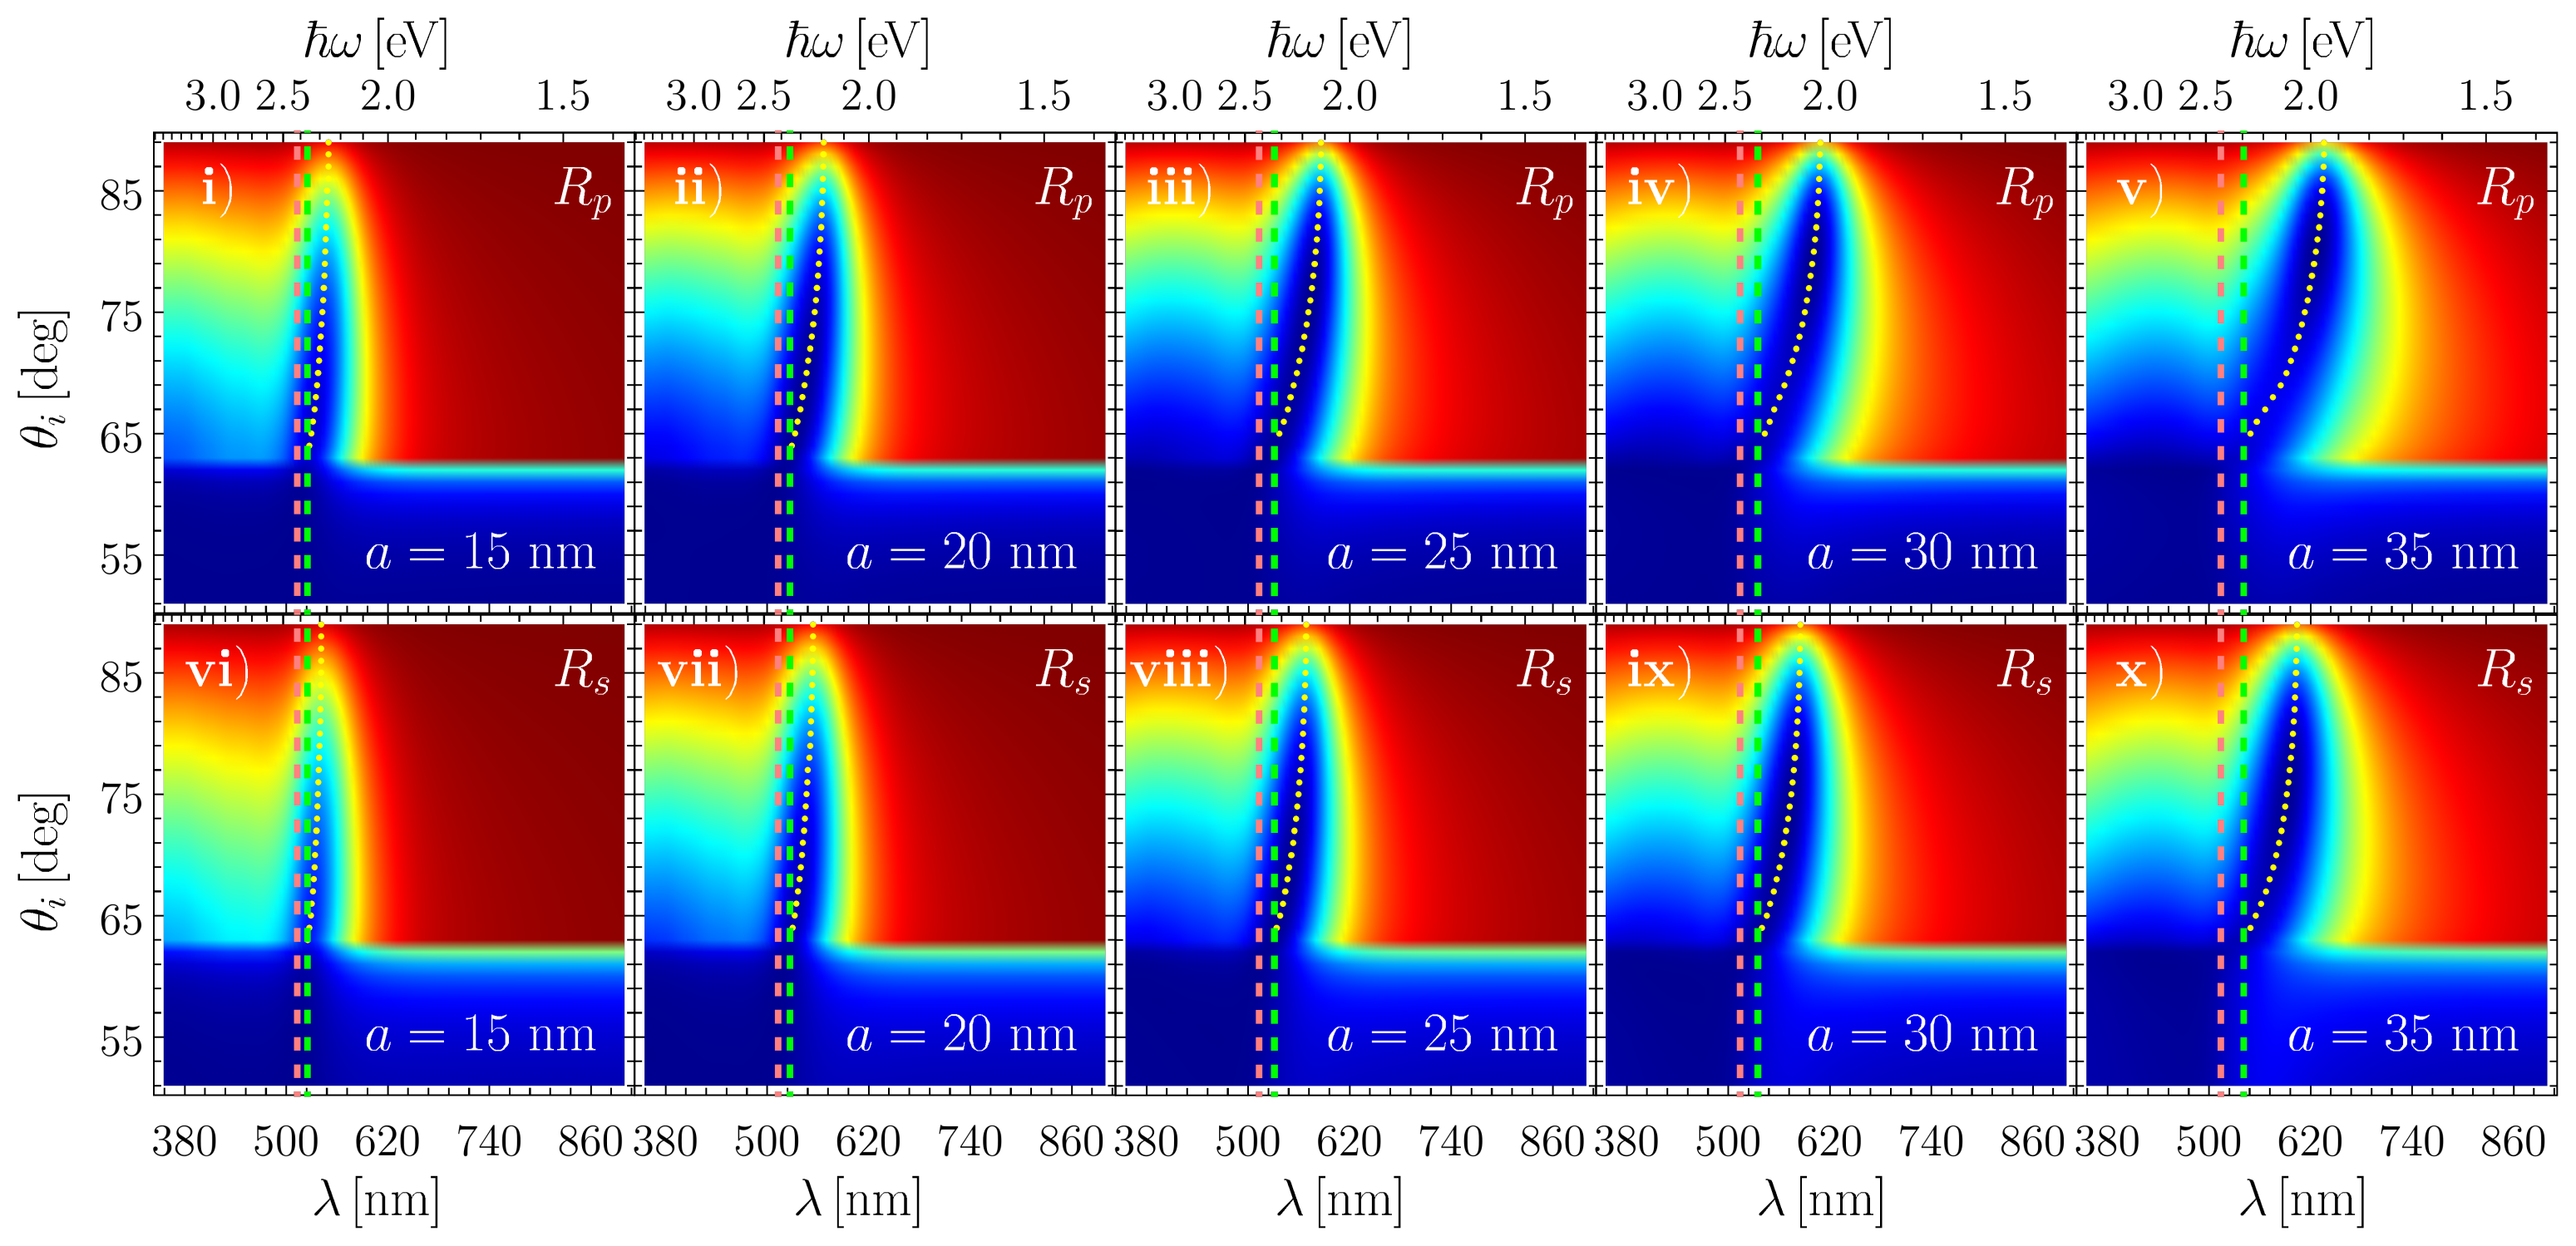
\includegraphics[width = .9\linewidth]{2-Resultados/figs/8-AurVar/0-2D_Grid}};
\node[right, inner sep=0pt] (legend) at (7,.05) {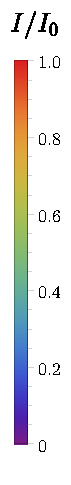
\includegraphics[scale=.78, trim={00 00 00 00}, clip]{2-Resultados/figs/0-IBar_v}};
\node[above, inner sep=0pt] (r) at (7.15,3.2) {$R$};
\end{tikzpicture}\vspace*{-.5em}
	\caption{Gráficas de reflectancia de una monocapa de NPs de oro en configuración ATR como función del ángulo de incidencia $\theta_i$ y de la longitud de onda $\lambda$ (escala inferior), así como de la energía  $\hbar\omega$ (escala superior).  Las gráficas   en el renglón superior [$\mathbf{i)-v)}$] muestran los resultados para  polarización \emph{p} y las del renglón inferior  [$\mathbf{vi)-x)}$]  para polarización  \emph{s}, donde se consideró una fracción de cubierta $\Theta = 0.123$ y  NPs de radio  $a$: $20$ nm, $25$ nm, $30$ nm y $35$ nm.  Las líneas verticales punteadas verdes y rosas corresponden a las SP-SPRs dipolar y  cuadrupolar, respectivamente.  Los puntos amarillos corresponden a los mínimos en $R$ para ángulos mayores a $\theta_c\approx 62.5^\circ$ y longitudes de onda mayores a la SP-SPRs dipolar.
}	\label{fig:Au-R-Rad}	
	\end{figure}	

Otra característica compartida por todos los casos estudiados de $\Theta$, al comparar los cortes para $\theta_i=65^\circ$ (Fig. \ref{fig:AuAg-Cuts-65}) y para $\theta_i=75^\circ$ (Fig. \ref{fig:AuAg-Cuts-75}), es una mejor definición del pico de la resonancia, así como su forma, como se observa al comarar los resultados para la monocapa de NPs de plata para los dos ángulos de incidencia escogidos, sobre todo para el caso de $\Theta=0.2$. De forma contraria, los valores de la reflectancia a $\lambda^{exc}$ no sigue un comportamiento análogo la plata con el oro: para las NPs de oro, $R_p\approx 0$ cuando $\Theta=0.125$ (línea naranja) y $R_s\approx 0$ para $\Theta=0.15$ (línea amarilla) mas para las NPs de plata $R\approx 0$, para ambas polarizaciones, cuando $\Theta=0.1$ (línea negra). Es decir, para los valores de fracciones de cubierta $\Theta$ escogidos, considerando NPs de oro de de $25$ nm y de plata de $35$ nm, la optimización de la monocapa para el biosensado es distinta.

Para determinar si los radios escogidos para las NPs de oro y de plata son los óptimos para el empleo del modo colectivo en el sensado, se presentan en la Fig. \ref{fig:Au-R-Rad}	gráficas de la reflectancia para una monocapa de NPs de oro, inmersa en un medio con $n_m=1.5$ y soportada por un sustrato con $n_s=1.5$ en configuración ATR. La fracción de cubierta de la monocapa es de $\Theta=0.125$, escogida con base en los resultados calculados en las Figs. \ref{fig:AuAg-Cuts-65} y \ref{fig:AuAg-Cuts-75}, y donde se varían los radios de las NPs al rededor de $35$ nm, es decir, $a=20$ nm, $25$ nm, $30$ nm y $35$ nm, siendo entonces las SP-SPR dipolares (líneas punteadas verticales verdes) $525$ nm, $527$ nm, $531$ nm, $535$ nm y $541$ nm para cada radio, respectivamente, y las cuadrupolares (líneas punteadas verticales rosas) $513$ nm para $a=15$ nm, $20$ nm y $25$ nm, y $514$ nm para $a=30$ nm y $35$ nm; el modo colectivo se representa mediante los punto amarillos.



En la Fig. \ref{fig:Au-R-Rad} se observa la tendencia identificada con la monocapa de NPs con una función dieléctrica tipo Drudo al variar el tamaño de las NPs: a radios $a$ mayores, el modo colectivo se corre al rojo y el ancho de la resonancia aumenta; conforme el radio disminuye, el modo colectivo tiende a reproducir a la SP-SPR dipolar. Al comparar la respuesta EM de la monocapa de NPs de oro ante variaciones de fracción de cubierta (Fig. \ref{fig:Au-R-Theta})  se observa que el modo colectivo (puntos amarillos) a la longitud de onda de la SP-SPR dipolar (línea punteada verde) se excita a un ángulo de incidencia $\theta_i$ para cada valor de $\Theta$ mas este valor no cambia para distintos valores de $a$, como se observa en la Fig. \ref{fig:Au-R-Rad}, en donde para ambas polarizaciones, el modo colectivo es apreciable para valores de $\lambda$ mayores o iguales a la del SP-SPR dipolar a partir de $\theta_i\approx 65^\circ$.

En la Fig. \ref{fig:Ag-R-Rad}	 se presentan los cálculos de la reflectancia de una monocapa de NPs  de plata, inmersa en un medio con $n_m=1.5$ y soportada por un sustrato con $n_s=1.5$ en configuración ATR. Se considera  $\Theta=0.1$,  según el análisis de las Figs. \ref{fig:AuAg-Cuts-65} y \ref{fig:AuAg-Cuts-75}, y los radios de las NPs al rededor de $35$ nm, es decir, $a=30$ nm, $35$ nm, $40$ nm, $45$ nm y $50$ nm, siendo entonces las SP-SPR dipolares (líneas punteadas verticales verdes) $417$ nm, $430$ nm, $44$ nm, $459$ nm y $479$ nm para cada radio, respectivamente, y las cuadrupolares (líneas punteadas verticales rosas) $373$ nm, $376$ nm, $379$ nm, $383$ nm y $388$ nm, respectivamente; el modo colectivo se representa mediante los punto amarillos.

\begin{figure}[h!]\centering
\begin{tikzpicture}
\node[inner sep=0pt] (graf) at (-.1,0){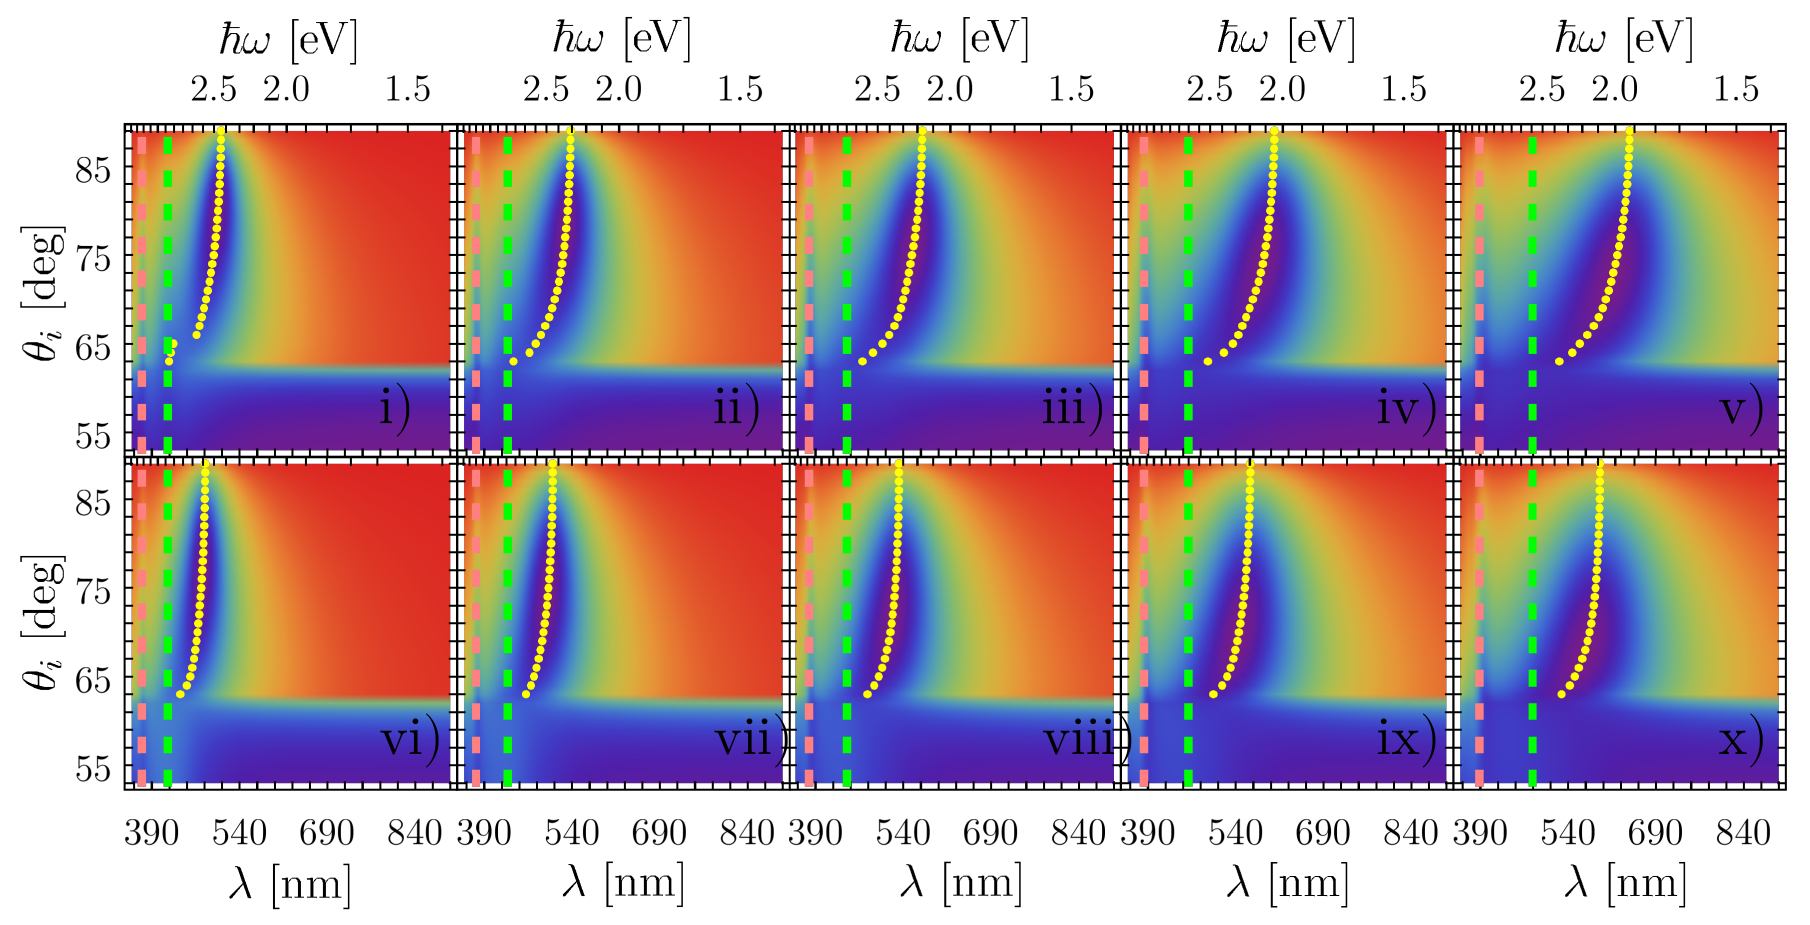
\includegraphics[width = .9\linewidth]{2-Resultados/figs/9-AgrVar/0-2D_Grid}};
\node[right, inner sep=0pt] (legend) at (7,.05) {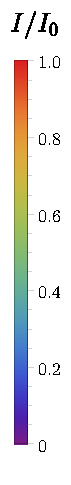
\includegraphics[scale=.78, trim={00 00 00 00}, clip]{2-Resultados/figs/0-IBar_v}};
\node[above, inner sep=0pt] (r) at (7.15,3.2) {$R$};
\end{tikzpicture}\vspace*{-.5em}
	\caption{Gráficas de reflectancia de una monocapa de NPs de plata en configuración ATR como función del ángulo de incidencia $\theta_i$ y de la longitud de onda $\lambda$ (escala inferior), así como de la energía  $\hbar\omega$ (escala superior).  Las gráficas   en el renglón superior [$\mathbf{i)-v)}$] muestran los resultados para  polarización \emph{p} y las del renglón inferior  [$\mathbf{vi)-x)}$]  para polarización  \emph{s}, donde se consideró una fracción de cubierta $\Theta = 0.1$ y  NPs de radio  $a$: $30$ nm, $35$ nm, $40$ nm, $45$ nm y $50$ nm.  Las líneas verticales punteadas verdes y rosas corresponden a las SP-SPRs dipolar y  cuadrupolar, respectivamente.  Los puntos amarillos corresponden a los mínimos en $R$ para ángulos mayores a $\theta_c\approx 62.5^\circ$ y longitudes de onda mayores a la SP-SPRs dipolar.
}	\label{fig:Ag-R-Rad}	
	\end{figure}	

La reflectancia de una monocapa de NPs de plata (Fig. \ref{fig:Ag-R-Rad}) para $\lambda\approx 300$ nm es cercana a la unidad para todos los radios $a$ considerados, comportamiento que también se observó en la Fig. \ref{fig:Ag-R-Theta} cuando se varió $\Theta$. Esta característica, presente sólo para la plata, puede emplearse para la caracterización del material empleado para las NPs de una monocapa. Para las longitudes de onda de las SP-SPRs, las excitaciones cuadrupolares (líneas verticales punteadas rosas) son más apreciables que las dipolares, para $\theta_i>\theta_c\approx 62.5^\circ$. Finalmente, respecto al  modo colectivo (puntos amarillos en la Fig. \ref{fig:Ag-R-Rad}) su comportamiento es semejante al observado para el oro en la Fig. \ref{fig:Au-R-Rad}: al aumentar el radio de las NPs, el modo colectivo es más apreciable y se corre hacia el rojo, efecto que se aprecia más para polarización \emph{p} que para \emph{s}.

Para comparar los resultados de la reflectancia al emplear la función dieléctrica de del oro y de la plata para las NPs, se grafican en la Fig. \ref{fig:AuAg-Cuts-Rad} cortes a $\theta_i = 65^\circ$ de la relfectancia $R$ de las Figs. \ref{fig:Au-R-Rad} y \ref{fig:Ag-R-Rad}. Las Figs. \ref{sfig:Au-cutp-Rad} y \ref{sfig:Au-cuts-Rad} son las gráficas de la reflectancia de una monocapa de NPs de oro con una onda plana incidiendo con polarización \emph{p} y \emph{s}, respectivamente, mientras que las Figs.  \ref{sfig:Ag-cutp-Rad} y\ref{sfig:Ag-cuts-Rad}  corresponden a la relfectancia de una monocapa de NPs de plata para polarización \emph{p} y \emph{s}, respectivamente. En todas las gráficas de la Fig. \ref{fig:AuAg-Cuts-Rad} la región sombreada verde corresponde al intervalo en $\lambda$ de las SP-SPRs para los radios $a=20$ nm, $30$ nm, $40$ nm y $50$ nm tanto para la excitación dipolar (región verde), como la cuadrupolar (rosa). 

\begin{figure}[h!]\centering\hspace*{-1.5em}
	\begin{subfigure}{.01\linewidth}\caption{}\label{sfig:Au-cutp-Rad}\vspace{4.5cm}\end{subfigure}
	\begin{subfigure}{.45\linewidth}\hspace*{-1.5em}
	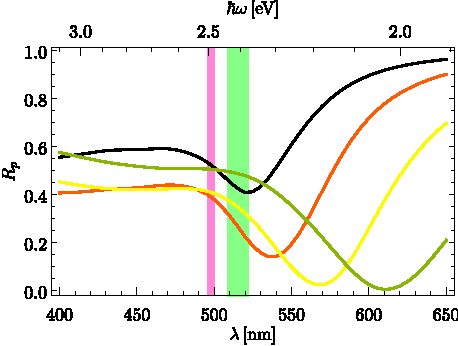
\includegraphics[scale=1]{2-Resultados/figs/8-AurVar/cut_angle_65_p.pdf}\end{subfigure}
	\begin{subfigure}{.01\linewidth}\caption{}\label{sfig:Au-cuts-Rad}\vspace{4.5cm}\end{subfigure}\hspace*{-1.em}
	\begin{subfigure}{.45\linewidth}\centering
	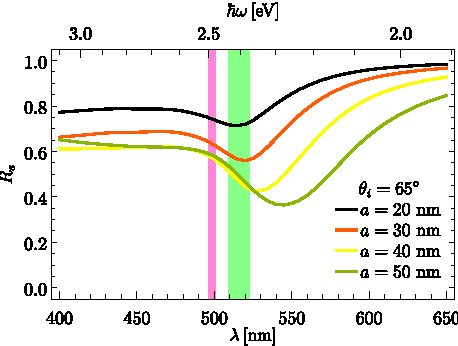
\includegraphics[scale=1 ]{2-Resultados/figs/8-AurVar/cut_angle_65_s.pdf}\end{subfigure}\vspace*{-0em}\\
	\hspace*{-1.5em}
	\begin{subfigure}{.01\linewidth}\caption{}\label{sfig:Ag-cutp-Rad}\vspace{4.5cm}\end{subfigure}
	\begin{subfigure}{.45\linewidth}\hspace*{-1.5em}
	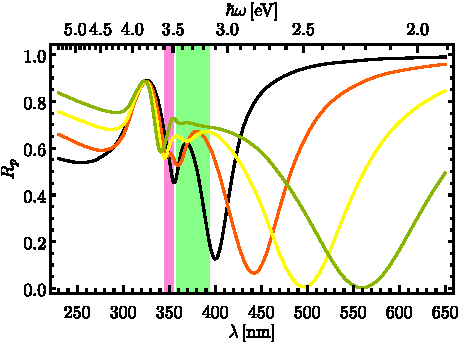
\includegraphics[scale=1]{2-Resultados/figs/9-AgrVar/cut_angle_65_p.pdf}\end{subfigure}
	\begin{subfigure}{.01\linewidth}\caption{}\label{sfig:Ag-cuts-Rad}\vspace{4.5cm}\end{subfigure}\hspace*{-1.em}
	\begin{subfigure}{.45\linewidth}\centering
	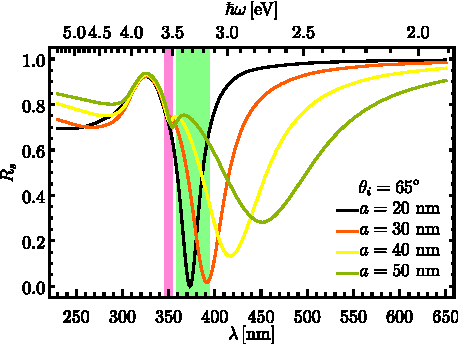
\includegraphics[scale=1 ]{2-Resultados/figs/9-AgrVar/cut_angle_65_s.pdf}\end{subfigure}\vspace*{-.5em}
	\caption{Cortes a $\theta_i = 65^\circ$ de las gráficas de reflectancia de una monocapa en configuración ATR (Fig. \ref{fig:R-RVar}) de NPs esféricas de fracción de cubierta $\Theta = 0.3$ en polarización \textbf{a)} \emph{p} y \textbf{b)} \emph{s} como función de la longitud de onda $\lambda$ (escala inferior) y de la energía $\hbar\omega$ (escala superior). Los parámetros de la función dieléctrica tipo Drude para las NPs son $\hbar\omega_p = 4.3$ eV y $\hbar\gamma = 0.15$ eV y las fracciones de cubierta consideradas fueron $a$: $3$ nm, $5$ nm, $10$ nm y $20$ nm. La SP-SPR dipolar para los tamaños de partículas utilizadas corresponde la región verde entre $500$ nm y $512$ nm, mientras que la cuadrupolar corresponde a la región rosa entre $456$ nm y $462$ nm.}\label{fig:AuAg-Cuts-Rad}
	\end{figure}	

Para el caso de una monocapa de NPs de oro [Figs. \ref{sfig:Au-cutp-Rad} y \ref{sfig:Au-cuts-Rad}], se presenta un mínimo en la reflectancia $R$ a longitudes de onda mayores a las de las SP-SPRs por lo que se identifica como el modo colectivo. Reproduciendo la tendencia observada para monocapas de NPs con una función dieléctrica tipo Drude, al aumentar el tamaño de las NPs, la excitación colectiva sufre un corrimiento al rojo en ambas polarizaciones: para polarización \emph{p} el modo colectivo se excita en el intervalo entre $520$ nm y $620$ nm y para polarización \emph{s} entre $510$ nm y $550$ nm. Al comparar el corrimiento al rojo al variar el radio de las NPs, con $\Theta=0.2$, y al variar la fracción de cubierta, con $a=30$ nm [ver Fig. \ref{fig:Au-R-Theta}], se observa que el corrimiento al rojo es mayor al considerar NPs más grandes que al considerar mayores fracciones de cubierta. De igual forma, los valores de la reflectancia a los valores de $\lambda$ del modo colectivo cumple con que  $R<0.2$ para $a\geq 30$ nm en polarización \emph{p} [ver Fig. \ref{sfig:Au-cutp-Rad}] y  para polarización \emph{s}  [ver Fig. \ref{sfig:Au-cuts-Rad}] $0.4<R<0.8$, que son valores menores a los observados en la variación de $\Theta$ en la Fig. \ref{fig:AuAg-Cuts}.

Respecto a la respuesta EM de una monocapa de NPs de plata, se observa en las Figs. \ref{sfig:Ag-cutp-Rad} y \ref{sfig:Ag-cuts-Rad} un máximo en la reflectancia en $\lambda \approx 330$ nm, que se apreciaba a distintos valores de $\Theta$ en la Fig. \ref{fig:AuAg-Cuts}. Al considerar el radio de las NPs variable pero la fracción de cubierta constante, se corrobora que el valor de $R_p$ y $R_s$ en $\lambda\approx 330$ nm es constante para un $\Theta$ fijo, por lo que puede emplearse esta longitud de onda para caracterizar la fracción de cubierta de una monocapa de NPs esféricas de plata; en particular para $\Theta=0.2$, $R_p = 0.9$ y $R_s = 0.95$ en $\lambda \approx 330$ nm. Una característica en común con la variación de $\Theta$, es que al aumentar el radio de las NPs de plata aún es apreciable la resonancia cuadrupolar de partícula individual considerando un corrimiento de esta excitación hacia le azul, como se observa en los mínimos en $R_p$ al rededor de la región rosa; en polarización \emph{s} la excitación cuadrupolar sólo es apreciable para $a=40$ nm y $50$ nm. La SP-SPR dipolar es también es apreciable para la polarización \emph{p} en la región de $360$ nm$<\lambda<390$ nm sin embargo, no es apreciable para la polarización \emph{s} dado que se traslapa con la excitación del modo colectivo. La excitación colectiva, al igual que se en caso de las NPs de oro, sufre un corrimiento al rojo mayor al aumentar el radio de las NPs que al aumentar la fracción de cubierta, además de disminuir el valores de $R$ al evaluarlo en la longitud de onda de la excitación colectiva: para polarización \emph{p} el modo colectivo se excita entre $400$ nm y $550$ nm, es decir que se sintoniza en la mitad del espectro visible, además de que para $20$ nm y $30$ nm $R_p<0.2$ y para $40$ nm y $50$ nm $R_p \approx 0$; para polarización \emph{s}, $R_s\leq 0.2$ al excitar el modo colectivo ($370$ nm$<\lambda<460$ nm) para $a\leq 40$ nm y $R_s\approx 0.4$ para $a=50$ nm.

\begin{figure}[h!]\centering
	\begin{subfigure}{.01\linewidth}\caption{}\label{sfig:RT-4}\vspace{6.5cm}\end{subfigure}
	\begin{subfigure}{.7\linewidth}\hspace*{-.5em}
	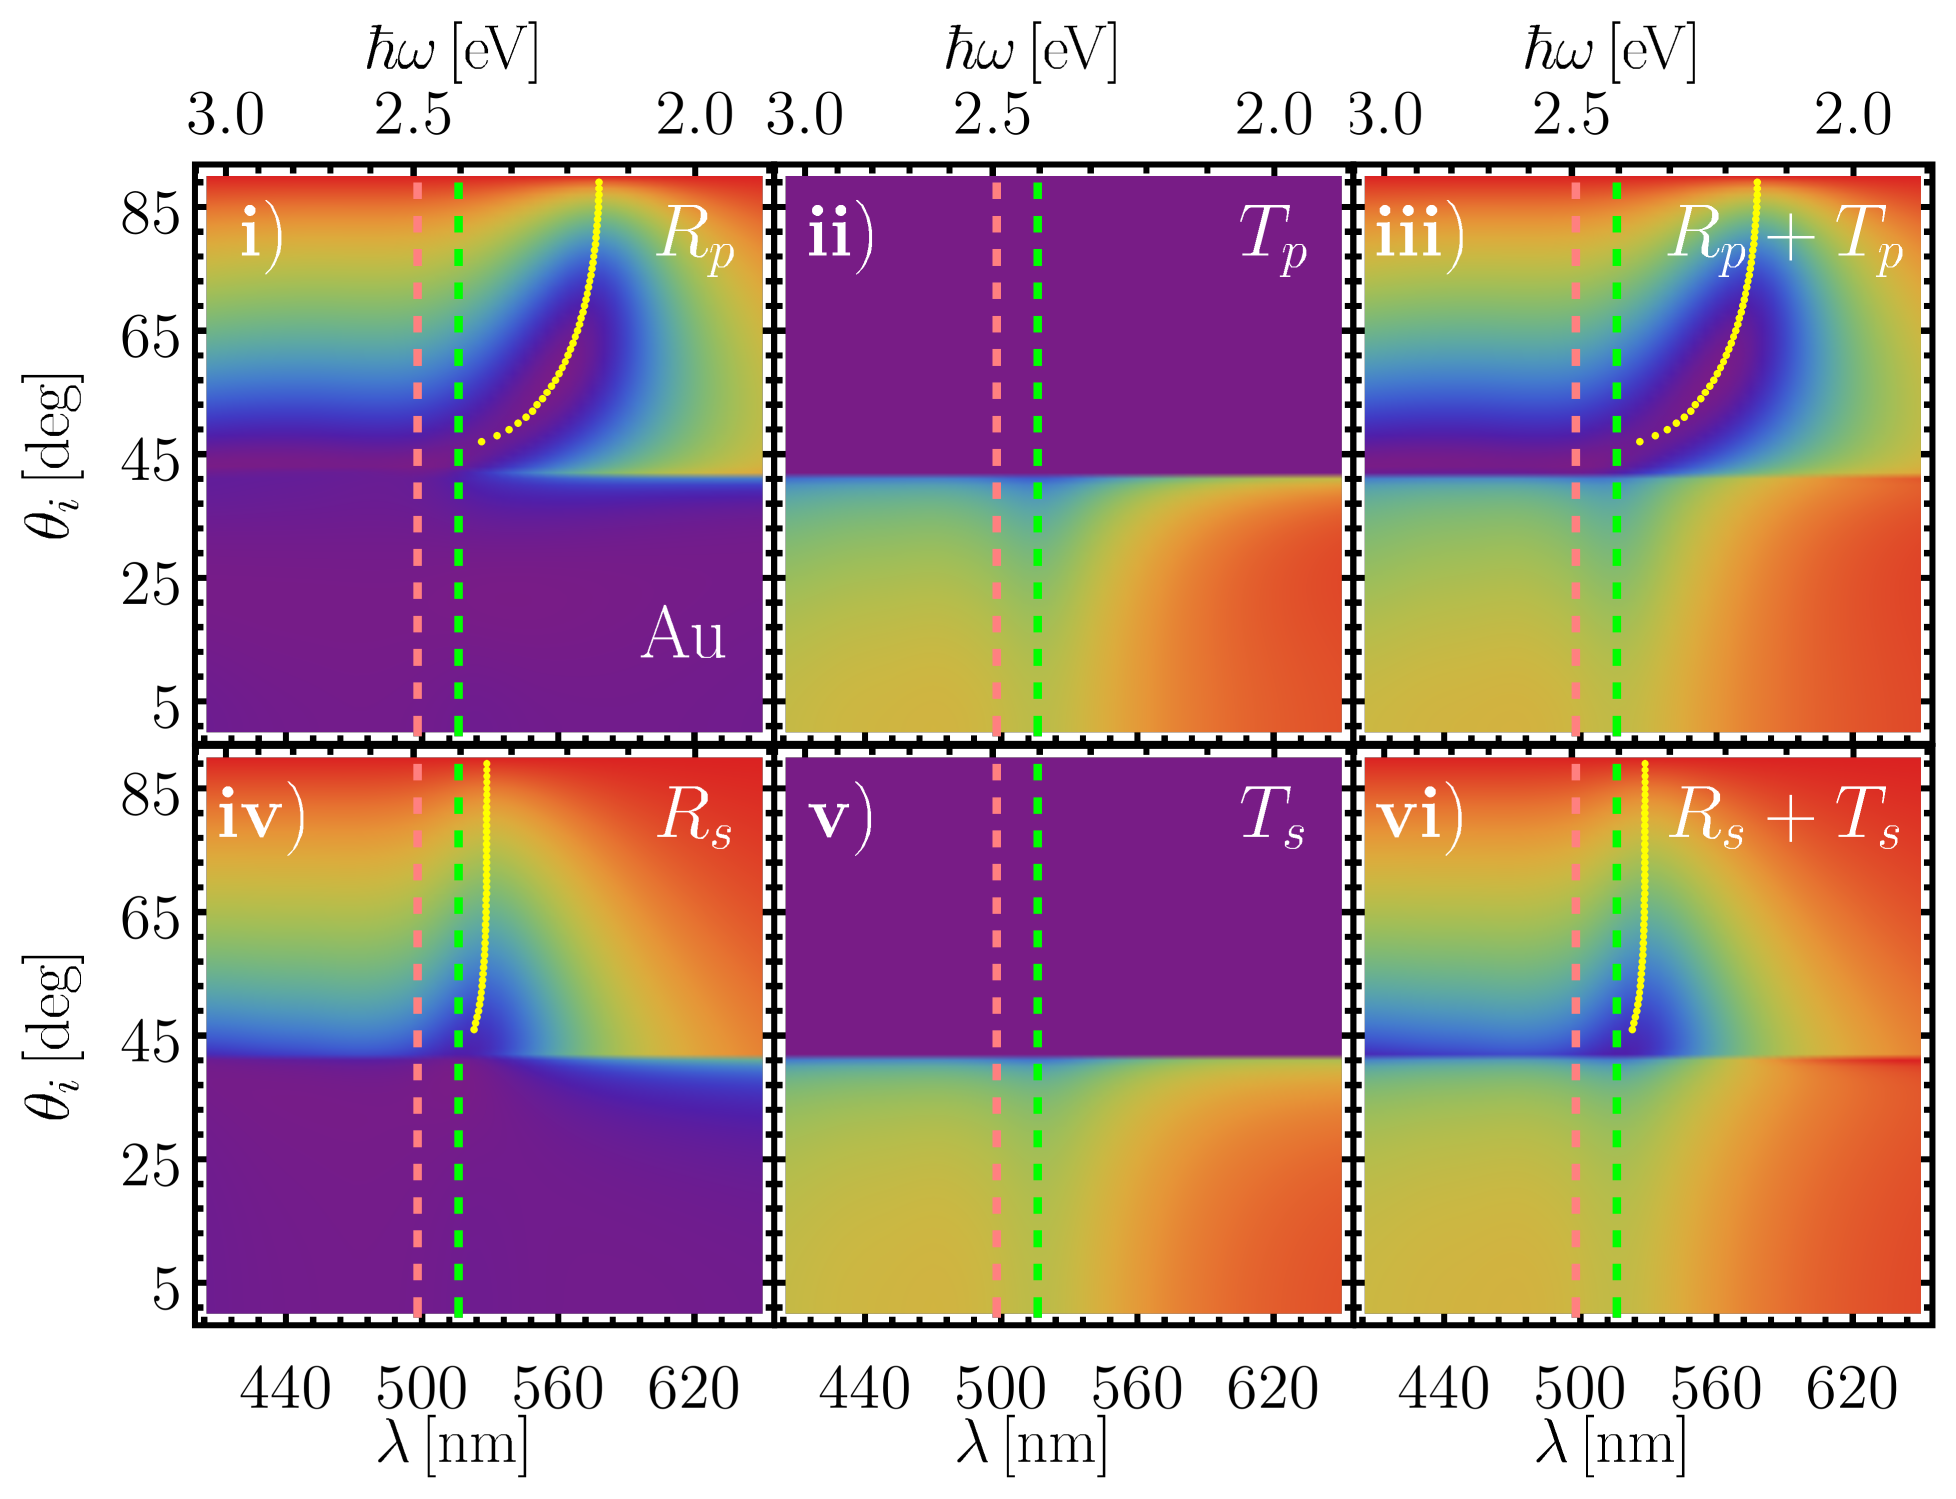
\includegraphics[scale=.58]{2-Resultados/figs/10-RT-AuAg/0-2D_Grid_1.png}%	
	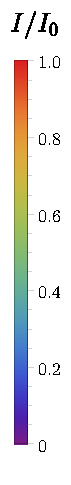
\includegraphics[scale=.89, trim={00 -5 00 00}, clip]{2-Resultados/figs/0-IBar_v}
	\end{subfigure}\\
	\begin{subfigure}{.01\linewidth}\caption{}\label{sfig:RT-10}\vspace{6.5cm}\end{subfigure}\hspace*{-1em}
	\begin{subfigure}{.7\linewidth}\centering
	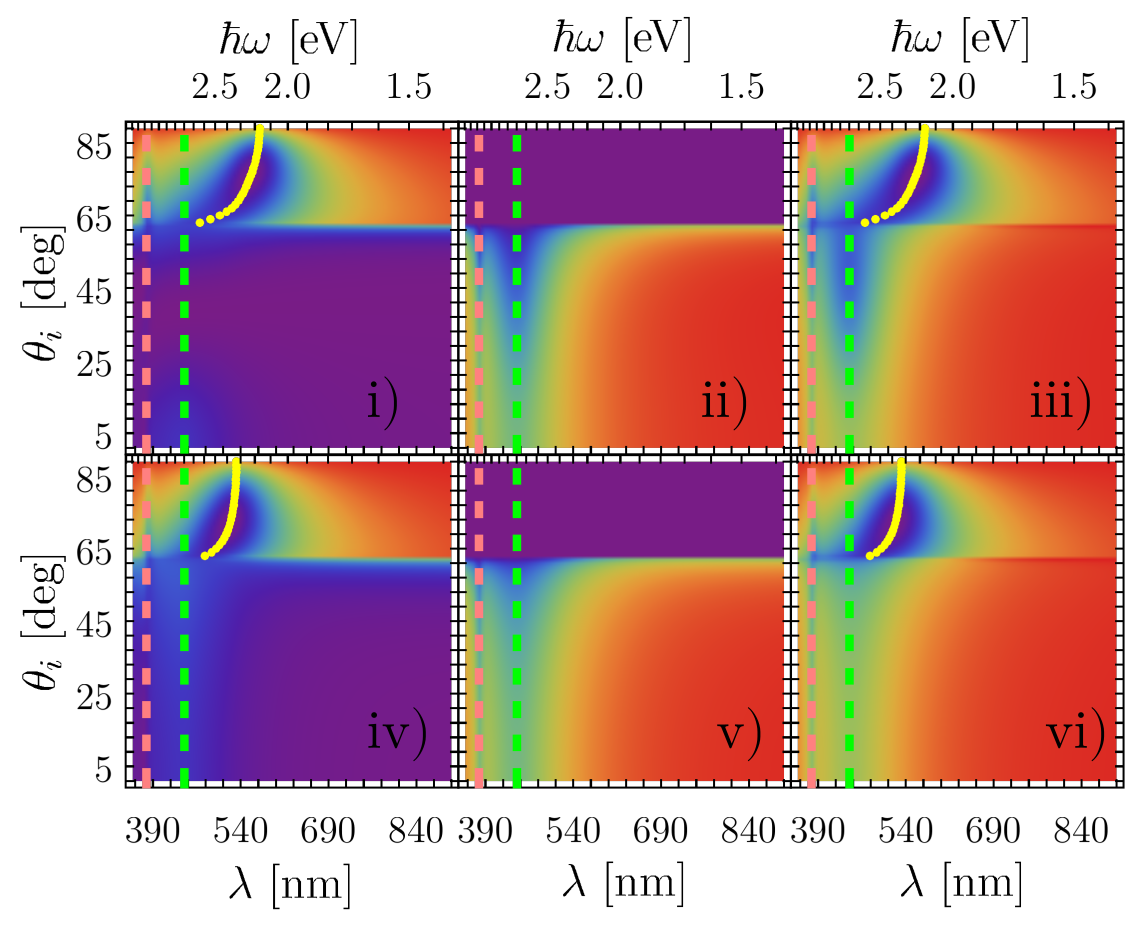
\includegraphics[scale=.58 ]{2-Resultados/figs/10-RT-AuAg/0-2D_Grid_2.png}%
		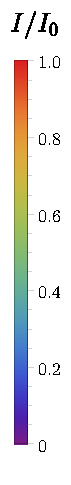
\includegraphics[scale=.89, trim={00 -5 00 00}, clip]{2-Resultados/figs/0-IBar_v}
		\end{subfigure}\vspace*{-.5em}
	\caption{Gráficas de reflectancia $R$, transmitancia $T$ y la suma de éstas $R+T$ de una monocapa en configuración ATR como función del ángulo de incidencia $\theta_i$ y de la longitud de onda $\lambda$ (escala inferior) así como de la energía del haz incidente en unidades de $\hbar\omega$ (escala superior), para una función dieléctrica tipo Drude con \textbf{a)} $\hbar\omega_p=4. 3$ eV  y  $\hbar\gamma=0. 15$ eV y \textbf{b)} $\hbar\omega_p = 10$ eV y $\hbar\gamma = 0.15$ eV.  Las gráficas   en el renglón superior [$\mathbf{i)-ii)}$]  muestran los resultados de reflectancia para  polarización \emph{p} y las del renglón inferior  [$\mathbf{iv)-vi)}$] para polarización  \emph{s}, donde se consideraron NPs de radio $a=30$ nm. Las líneas verticales punteadas verdes corresponden a la SP-SPRs dipolar ($526$ nm y $265$ nm para $\hbar\omega_p=4.3$ eV y $\hbar\omega_p = 10$ eV, respectivamente), las rosas a la SP-SPR cuadrupolar ($462$ nm y $211$ nm para $\hbar\omega_p=4.3$ eV y $\hbar\omega_p = 10$ eV, respectivamente) y las cianes a la SP-SPR octopolar ($195$ nm para $\hbar\omega_p = 10$ eV). Los puntos amarillos corresponden a los mínimos en $R$, y $R+T$ para ángulos mayores a $\theta_c\approx 41.8^\circ$ y longitudes de onda mayores a la SP-SPRs dipolar. }\label{fig:RT-Omegas}
	\end{figure}	





La construcción de un sensor para materia biológica basado en la respuesta EM colectiva de una monocapa de NPs plasmónicas es posible al emplear oro o plata, según los resultado de la reflectancia graficados en la Fig. \ref{fig:AuAg-Cuts}.  En l




